\documentclass{article}
\usepackage{graphicx} % Required for inserting images
\usepackage{mathrsfs}

\title{ECE148: Signal Processing Applications \\\large 
        Assignment 3: System Conversion}
\author{Andy Chen}
\date{April 2026}

\begin{document}

\maketitle

\section{Introduction}
Consider a simple 2nd-order analog system defined by the differential equation:
\[
(D^2 + \beta^2) y(t) = \beta x(t)
\]
where \(\beta\) is a real and positive scalar.

\section{Transfer Function \(H(s)\) and Impulse Response \(h(t)\)}
Taking the Laplace transform of the differential equation yields:
\[
(s^2 + \beta^2)Y(s) = \beta X(s)
\]
After some manipulation, we have the transfer function \(H(s)\):
\[
H(s) = \frac{Y(s)}{X(s)} = \frac{\beta}{s^2 + \beta^2}
\]
The inverse Laplace transform of the transfer function is simply the impulse response \(h(t)\):
\[
h(t) = \mathscr{L}^{-1} \{ \frac{\beta}{s^2 + \beta^2} \} = \sin(\beta t) \ u(t)
\]

\section{Equation Conversion Method}
\subsection*{Difference Equation}
Using:
\[
D \approx \frac{1-z^{-1}}{\Delta t} \Rightarrow D^2 \approx \frac{(1-z^{-1})^2}{\Delta t^2}
\]
Substituting into the differential equation yields:
\[
(\frac{(1-z^{-1})^2}{\Delta t^2} + \beta^2) Y(z) = \beta X(z)
\]
\[
(\frac{1-2z^{-1} + z^{-2}}{\Delta t^2} + \beta^2) Y(z) = \beta X(z)
\]
\[
(\frac{1}{\Delta t^2} + \beta^2 - \frac{2}{\Delta t^2} z^{-1} + \frac{1}{\Delta t^2} z^{-2} ) Y(z) = \beta X(z)
\]
Taking the inverse Z-transform:
\[
(\frac{1}{\Delta t^2} + \beta^2) y[n] - \frac{2}{\Delta t^2} y[n-1]+ \frac{1}{\Delta t^2} y[n-2] = \beta x[n]
\]

\subsection*{Transfer Function \(H(z)\)}
\[
H(z) = \frac{Y(z)}{X(z)} = \frac{\beta}{\frac{1}{\Delta t^2} ( 1-2z^{-1}+z^{-2}) + \beta^2}
\]
\[
H(z) = \frac{\beta \Delta t^2}{(1 + \beta^2 \Delta t^2)- 2z^{-1} + z^{-2}}
\]

\subsection*{Impulse Response \(h[n]\)}
Given the transfer function \(H(z)\):
\[
H(z) = \frac{z^2 \beta \Delta t^2}{z^2 (1+\beta^2 \Delta t^2) -2z + 1}
\]
We solve for the poles of \(H(z)\):
\[
z = \frac{2 \pm \sqrt{4-4(1+\beta^2 \Delta t^2)}}{2(1+\beta^2 \Delta t^2)}
\]
\[
z = \frac{2 \pm \sqrt{-4\beta^2 \Delta t^2}}{2(1+\beta^2 \Delta t^2)}
\]
\[
z = \frac{2 \pm 2j \beta \Delta t}{2(1+\beta^2 \Delta t^2)}
\]
\[
z = \frac{1 \pm j \beta \Delta t}{1+\beta^2 \Delta t^2}
\]

\[
|z| = \frac{\sqrt{1 + \beta^2 \Delta t^2}}{1+\beta^2 \Delta t^2} = \frac{1}{\sqrt{1 + \beta^2 \Delta t^2}} < 1
\]
\[
\theta = \tan^{-1}(\beta \Delta t)
\]
The magnitude of \(z\) is less than 1, so the pole is inside the unit circle. The system is stable. Note that the poles of \(z\) have an associated phase. We can therefore represent the pole as a complex exponential:
\[
z = \frac{1}{\sqrt{1+\beta^2 \Delta t^2}}e^{j \tan^{-1}(\beta \Delta t)}
\]
Rewriting \(H(z)\):
\[
H(z) = \frac{z^2 \beta \Delta t^2}
{(z - \frac{1}{\sqrt{1+\beta^2 \Delta t^2}}e^{j \tan^{-1}(\beta^ \Delta t)})(z - \frac{1}{\sqrt{1+\beta^2 \Delta t^2}}e^{-j \tan^{-1}(\beta \Delta t)})}
\]
\[
H(z) = \frac{z^2 \beta \Delta t^2}
{z^2 - z(\frac{1}{\sqrt{1+\beta^2 \Delta t^2}})(e^{j \tan^{-1}(\beta \Delta t)}+e^{-j \tan^{-1}(\beta^ \Delta t)}) + \frac{1}{1 + \beta^2 \Delta t^2} }
\]
\[
H(z) = \frac{z^2 \beta \Delta t^2}{z^2 - 2z(\frac{1}{\sqrt{1+\beta^2 \Delta t^2}}) \cos(\tan^{-1}(\beta \Delta t)) + \frac{1}{1+\beta^2 \Delta t^2} }
\]
\[
H(z) = z \frac{\beta \Delta t^2 \sqrt{1+\beta^2 \Delta t^2}}{\sin(\tan^{-1}(\beta \Delta t))} 
\frac{z(\frac{1}{\sqrt{1+\beta^2 \Delta t^2}})\sin(\tan^{-1}(\beta \Delta t)) }{z^2 - 2z(\frac{1}{\sqrt{1+\beta^2 \Delta t^2}}) \cos(\tan^{-1}(\beta \Delta t)) + \frac{1}{1+\beta^2 \Delta t^2} }
\]
After matching with the z-transform pair, we get:
\[
h[n] = \frac{\beta \Delta t^2 \sqrt{1+\beta^2 \Delta t^2}}{\sin(\tan^{-1}(\beta \Delta t))}
(\frac{1}{\sqrt{1+\beta^2 \Delta t^2}})^{n+1} \sin(\tan^{-1}(\beta \Delta t)(n+1)) \ u[n+1]
\]
\[
h[n] = \frac{\beta \Delta t^2 \sqrt{1+\beta^2 \Delta t^2}}{\frac{\beta \Delta t}{\sqrt{1+\beta^2 \Delta t^2}}}
(\frac{1}{\sqrt{1+\beta^2 \Delta t^2}})^{n+1} \sin(\tan^{-1}(\beta \Delta t)(n+1)) \ u[n+1]
\]
\[
h[n] = \Delta t (1 +\beta^2 \Delta t^2)
(\frac{1}{\sqrt{1+\beta^2 \Delta t^2}})^{n+1} \sin(\tan^{-1}(\beta \Delta t)(n+1)) \ u[n+1]
\]
\pagebreak 

\begin{figure}
    \centering
    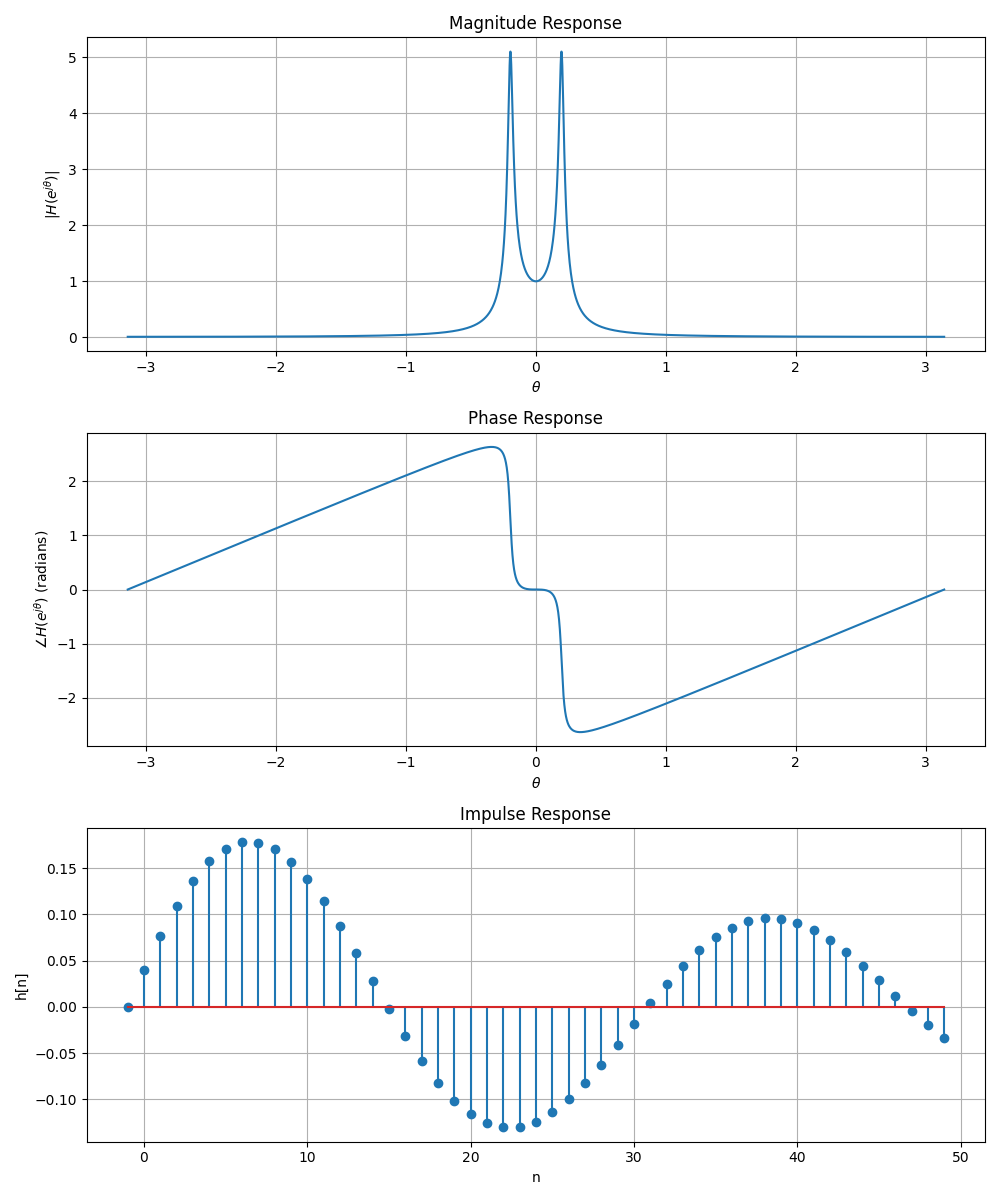
\includegraphics[width=1\linewidth]{equationconversionplot.png}
        \caption{Plot of frequency response \(H(e^{j\theta})\) and impulse response \(h(n)\)}
    \label{fig:placeholder}
\end{figure}

\section{Impulse Invariance Method}
\subsection*{Impulse Response \(h(n)\)}
Given the impulse response of the analog system:
\[
h(t) = \sin (\beta t) \ u(t)
\]
The impulse response of the discrete system is a sampling of the continuous impulse response:
\[
h[n] = \sin(\beta n\Delta t) \ u[n]
\]

\subsection*{Transfer Function \(H(z)\)}
Taking the impulse response of the discrete system and applying some manipulations:
\[
h[n] = \frac{1}{2j}(e^{j\beta \Delta t})^n - \frac{1}{2j}(e^{-j\beta \Delta t})^n \ u[n]
\]
We have the corresponding transfer function:
\[
H(z) = \frac{1}{2j} \frac{z}{z-e^{j\beta \Delta t}} - \frac{1}{2j} \frac{z}{z-e^{-j\beta \Delta t}}
\]

\subsection*{Difference Equation}
We manipulate the transfer function:
\[
H(z) = \frac{1}{2j} \frac{z(e^{j\beta \Delta t}-e^{-j\beta \Delta t})}{z^2 - z(e^{j\beta \Delta t} + e^{-j\beta \Delta t}) + 1}
\]
\[
H(z) = \frac{z\sin(\beta \Delta t)}{z^2 - 2z\cos(\beta\Delta t) + 1}
\]
\[
H(z) = \frac{Y(z)}{X(z)} = \frac{z^{-1}\sin(\beta \Delta t)}{1 - 2z^{-1}\cos(\beta\Delta t) + z^{-2}}
\]
\[
(1 - 2z^{-1}\cos(\beta\Delta t) + z^{-2})Y(z) = z^{-1}\sin(\beta \Delta t) X(z)
\]
We convert and solve for the difference equation:
\[
y[n] - 2\cos(\beta\Delta t) y[n-1]+y[n-2] = sin(\beta\Delta t)x[n-1]
\]
\begin{figure}
    \centering
    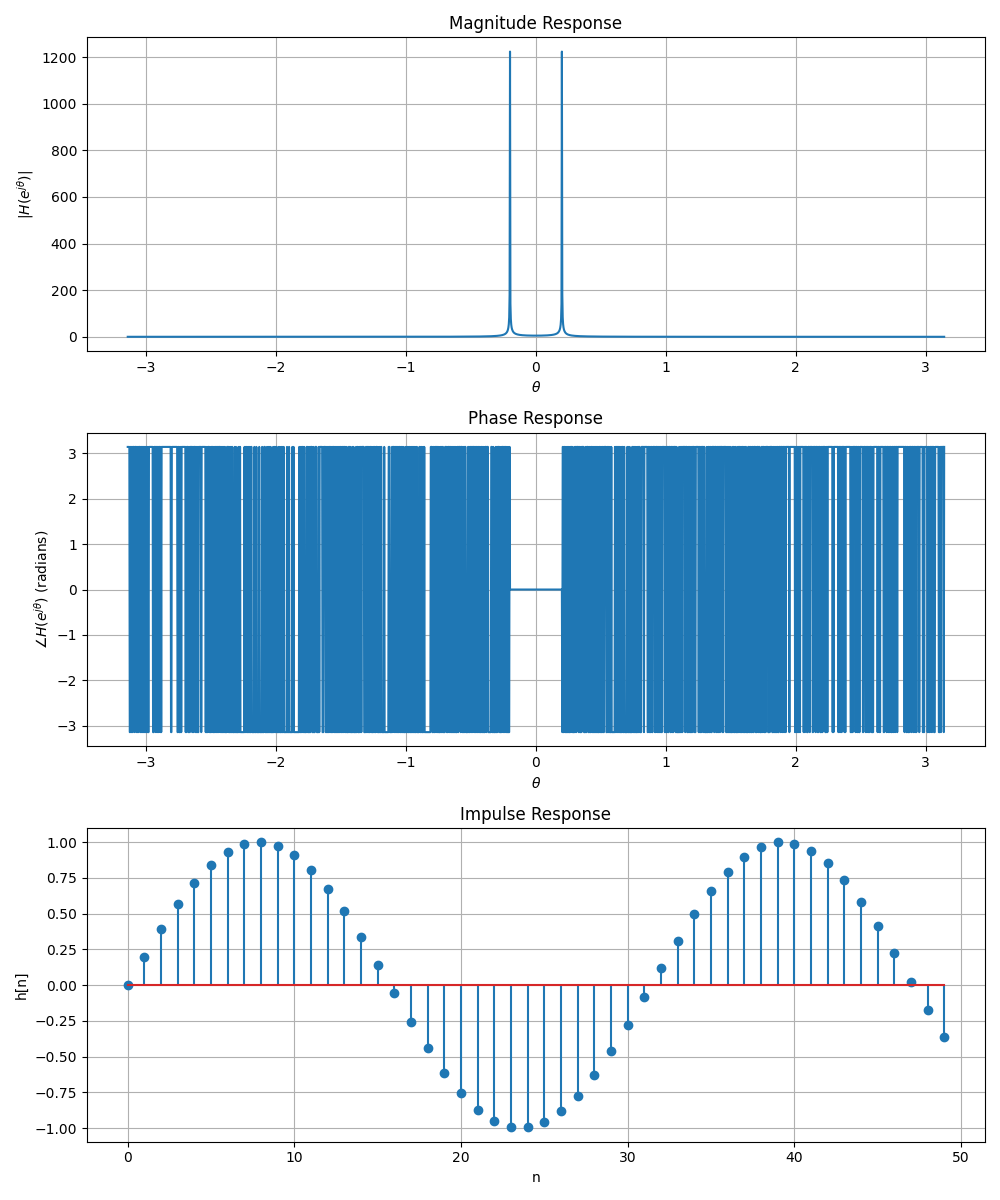
\includegraphics[width=1\linewidth]{impulseinvariancemethod.png}
    \caption{Plot of frequency response \(H(e^{j\theta})\) and impulse response \(h(n)\)}
    \label{fig:placeholder}
\end{figure}

\section{Pole Comparison (Equation Conversion vs. Impulse Invariance Methods)}
From the equation conversion method, we have the magnitude of the pole:
\[
|z| = \frac{1}{\sqrt{1+\beta^2 \Delta t^2}}
\]
From the impulse invariance method, we have the magnitude of the pole \(|z| = 1\). Therefore, the radial displacement of the two poles as a function of \(\Delta t\) is:
\[
\Delta z = 1 - \frac{1}{\sqrt{1+\beta^2 \Delta t^2}}
\]
From the equation conversion method, we have the phase of the pole \(\theta = \tan^{-1}(\beta \Delta t)\). From the impulse invariance method, we have the phase of the pole \(\theta = \beta\Delta t\). The angular displacement of the two poles as a function of \(\Delta t\) is therefore:
\[
\Delta \theta = \beta\Delta t - \tan^{-1}(\beta \Delta t)
\]
For small sampling intervals \(\Delta t\), both methods produce nearly identical pole locations. However, as \(\Delta t\) increases, the equation conversion poles move inward while the impulse invariance poles remain on the unit circle. The angular separation between the methods increases. Therefore, the equation conversion method introduces damping, while the impulse invariance method preserves the oscillatory nature of the original analog system.

\begin{figure}
    \centering
    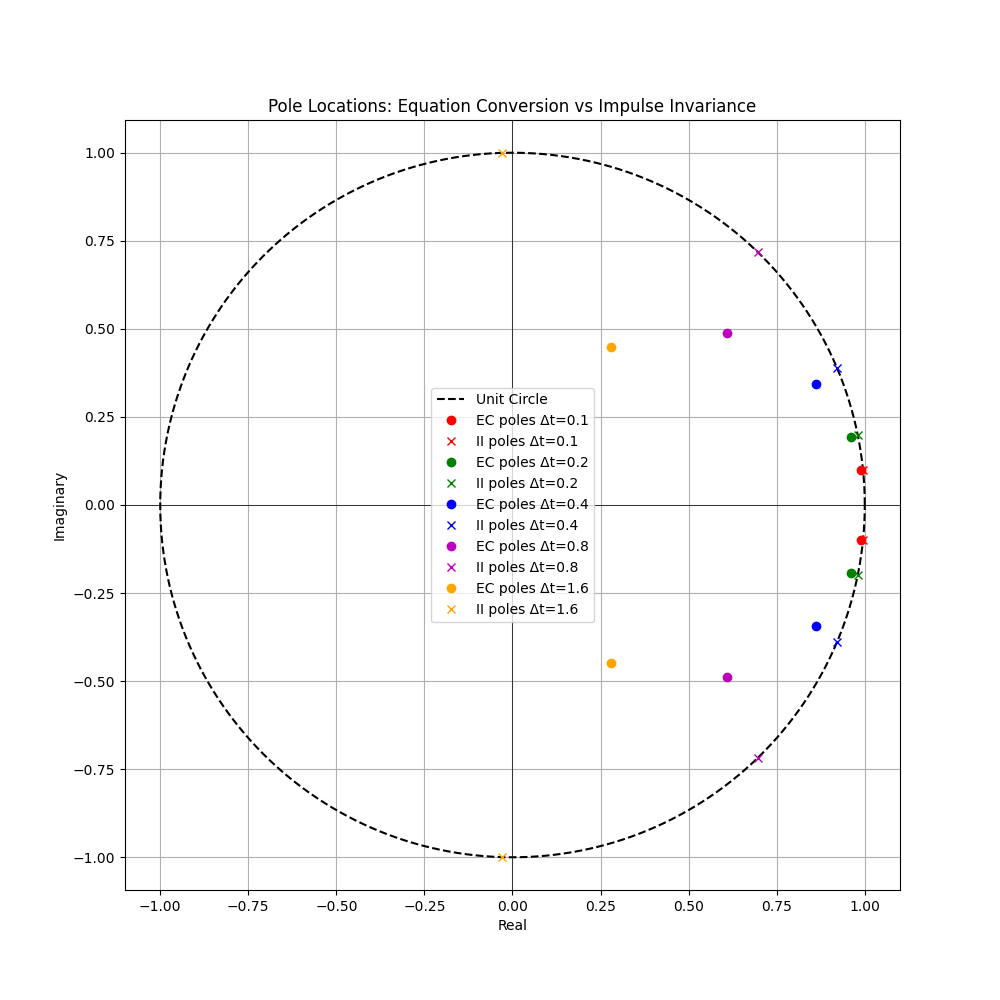
\includegraphics[width=1\linewidth]{polecomparison.png}
    \caption{Pole comparison of equation conversion and impulse invariance methods}
    \label{fig:placeholder}
\end{figure}

\end{document}
